  
\documentclass[titlepage]{article}
\usepackage[utf8]{inputenc}
\usepackage{amsmath}
\usepackage{tcolorbox}
\usepackage{amssymb}
\usepackage{amsthm}
\usepackage{empheq}
\usepackage{xcolor}
\usepackage{float}
\usepackage[
top    = 2.50cm,
bottom = 2.50cm,
left   = 2.75cm,
right  = 2.75cm]{geometry}
\usepackage{fancyhdr}
\pagestyle{fancy}
\lhead{Analysis 1}
\rhead{EPFL/Alp Ozen}

\newtheorem{remark}{Remark}[section]
\newtheorem{theorem}{Theorem}[section]
\newtheorem{prop}{[Proposition]}
\newtheorem{definition}{Definition}
\numberwithin{equation}{subsection}

\title{\textbf{Analysis 1 - Zsolt Patavflaki}}
\author{Alp Ozen}
\date{Fall 2019}
\newtheorem{example}{Example}[section]
\newtheorem{axiom}{Axiom}
\newtheorem{cor}{Corollary}

\begin{document}

\maketitle
\tableofcontents
\clearpage
\section{Proofs and the reals}
\subsection{Some general proofs}
A valid proof is set of lines where each line logically follows from the next. 
A most famous proof is that $\sqrt{2} $ is irrational. 

\begin{tcolorbox}
\begin{proof}
	Suppose that $\sqrt{2} = \frac{a}{b}$ where $a,b \in \mathbb{Z}$ and $gcd(a,b) = 1$
	\\
	Now we have that $\sqrt{2}b = a$ which means that $2b^2 = a^2$.
	As result, $2 \vert a^2$ hence also $2 \vert a$. Thus we get that $a = 2k$ which also means that $b^2 = 2k^2$ hence $2 \vert b$. As result, $gcd(a,b) = 2$ which is a contradiction. Therefore, $\sqrt{2}$ must be irrational. 
	\end{proof}
\end{tcolorbox}

Quite interestingly, we can also construct a 'wrong' proof just through one fallacious assumption and a set of correct steps. 

\begin{tcolorbox}
    \textbf{Claim:} 1 is the largest integer.
    \\
    Proof: 
    \\
    Let $n$ be the largest integer. Then we have $n \geq n^2$. Which also means $0 \geq n^2 - n = n(n-1)$. Now we have that either $n < 0$ or $n - 1 < 0$. But we know that $ n \nless 0$ as $n$ is at least 1. Hence, $n - 1 < 0$ giving us the result $n < 1$ proving our theorem. Note that the mistake here is solely the assumption we made at the start that there was a largest integer. 
\end{tcolorbox}
\subsection{Proofs relating to infinite processes}
Consider the claim that $0.999\ldots = 1$.
One way to prove this claim, rather naively is this.

\begin{align*}
    9 \times 0.999\ldots \\
    = (10 - 1) \times 0.999\ldots\\
    = 9.999\ldots - 0.999\ldots 
    = 1
\end{align*}

Now a more formal proof is to use an infinite sum and limits. Here it is. 

\begin{tcolorbox}
\textbf{Analysis proof of 0.999\ldots = 1}
    \begin{align*}
        0.999\ldots = 9\lim_{k\to\infty}\sum_{i=1}^{k} (10^{-k})\\
        \lim_{k\to\infty}\sum_{i=1}^{k}(10^{-k}) = \frac{10^{-1} - 10^{-(k+1)}}{1-10^{-1}}\\
        = 9 \times \frac{1}{10} \times \frac{10}{9}\\
        = 1
    \end{align*}
\end{tcolorbox}

\subsection{Basic notions of sets}
The breakdown of sets used in 'standard' analysis are $\mathbb{N} \subseteq \mathbb{Z} \subseteq \mathbb{Q} \subseteq \mathbb{R}$.
\\
There are also some common set related notation that must be known. 
\begin{itemize}
    \item a \textbf{subset} $a \subseteq b$ is defined as $\{x \in b \vert \text{"condition"}\}$
    \item a \textbf{open interval} is defined as $\left]a,b[; r\in A, a < r < b$
    \item an \textbf{open ball} $B(a,\lambda) = \left]a-\lambda,a+\lambda[$
\end{itemize}

\subsection{The Reals}

The reals, denoted \mathbb{R} are an ordered field. Here is a more precise definition.

\begin{tcolorbox}
The reals are a set that have the 3 following axioms:
\begin{itemize}
    \item \mathbb{R} is an abelian group under (+) and \mathbb{R*} is an abelian group under ($\times$). In addition to this, multiplication distributes over addition.
    \item The order relation $\leq$ holds $\forall x \in \mathbb{R}$ That is:
    \begin{align*}
        x \leq y \otimes y \leq x\\
        x \leq y, y \leq x \implies x = y\\
        x \leq y \implies \forall a \in \mathbb{R},\  x + a \leq y + a\\
        0 \leq x, 0 \leq y \implies 0 \leq xy
    \end{align*}
    \item The inf and sup axioms hold
\end{itemize}

We shall now come the \textbf{inf} and \textbf{sup} axioms. It should be intuitively clear that any subset of \mathbb{R} 
\end{tcolorbox}

\subsection{Bounds}
Take some subset S in \mathbb{R}. An element B is called an upper bound of S if $\forall x \in S, B \geq x$. Similarly, it is a lower bound of S if $\forall x \in S, B \leq x$.
\\
The maximum B of a set S denoted $max(S)$ is such that $B \in S, \forall x \in S, \ B \geq x$. 
\\
The supremum of a set S(if it exists) is the lowest upper bound. That is $sup(S) = b$ is such that,


    \begin{align}
        \forall x \in S, b \geq x\\
        \forall \epsilon > 0, \exists x_{\epsilon}, b - x_{\epsilon} \leq \epsilon
    \end{align}
    
    
    
    
    
\begin{remark}

   In our above definition, b does not have to be in S.

\end{remark}


\begin{remark}
    Condition 1 states that b is an upper bound of S. 
 
\end{remark}


\begin{remark}
       Given condition 1, b is the \textit{minimum} of the upper bounds of S.
\end{remark}
    
Some examples of $sup$ and $inf$

\begin{example}
\begin{align*}
 Sup ]a,b[ = b\\
 Inf ]a,b[ = a\\
 Sup \{ x\in \mathbb{R} \vert x = 2k\} \implies \text{Sup doesn't exist.}
\end{align*}
\end{example}


We now establish the infinimum axiom.
\begin{axiom}
All non-empty subsets of $\mathbb{R}_{+}^{*}$ have a highest lower boundary(aka.infinimum)
\end{axiom}

\subsection{\mathbb{Q} is dense in \mathbb{R}}
We claim that between every real number, one can find a rational number. Here's the proof,

\begin{tcolorbox}
\begin{proof}
    Let $x<y \in \mathbb{R}$ Suppose now that $\exists a \in \mathbb{Q}$ such that $x<a<y$. By the Archimedean principle(there is always a greater natural number, $n > \frac{1}{y-x}$ which implies $ny>nx+1$ Now since $ny>nx+1$, there is guaranteed to be some integer in the open bound $]nx,ny[$ which we denote $P$. Dividing by $n$, we get that $\frac{P}{n} \in ]x,y[$ which proves the theorem. 
    \tag*{\qedhere}
\end{proof}
\end{tcolorbox}

\subsection{Integer and fractional part}

Any number $\in \mathbb{R}$ has a integer and fractional part(at least intuitively). Let's formally define these. For some $x \in \mathbb{R}$, let $S := \{n\in\mathbb{N} \vert n > x\}$ Now since $S$ is bounded from below, letting $N$ be the minimum of this set, we obtain that $N \not\in S$. N-1 is thus called the integer part of x denoted [x]. ie. [6.4] = 6
\\
Similarly, the fractional part of x denoted {x} is simply ${x} = x - [x]$

\subsection{Pinning it down:Sup/Inf, bounds, max/min}
\begin{definition}
for a given set $S \subseteq \mathbb{R}$, we have the following:
\\
\textbf{Sup s = b} $\iff \forall \epsilon > 0, \exists x_{\epsilon} \in S, s.t. b - x_{\epsilon} < \epsilon$ (resp. Inf s has the flipped argument)
\\
\textbf{Upper bound = b} $\iff \forall x \in S, b\geq x$(resp. lower bound)
\\
\textbf{Max s = b} $\iff$ b is an upper bound and $b \in S$

\end{definition}
\\

And for the sake of repeating the early axiom(but very important) the infimum axiom is:
\begin{axiom}
For all non-empty subsets of $\mathbb{R}$, $inf S$ exists. 
\end{axiom}

Now we make the first claim in this course that uses an epsilon proof.
\begin{tcolorbox}

\begin{prop}
Whenever $S \subseteq \mathbb{N}$, then $inf S = min S$
\end{prop}

\begin{proof}
    Now, by our axiom, we have that $\mathbb{N} \subseteq \mathbb{R}$ hence we know that $inf S$ exists. We now have to show that $inf S = min S$. 
    \\
    
    Suppose that $inf S \not =  min S$ and let $inf S = b$. Now clearly, $b+\epsilon$ is not a lower bound of S. Now, let $\epsilon = \frac{1}{2}$. Because, $b + \epsilon$ is not a lower bound, we know that $\exists s_{e} < b + \epsilon$. 
    \\
    
    Now $s_{e$ is also not a lower bound, so let's pick $\epsilon^{\prime\prime} = s_{\epsilon} - d$. Now again, $s_{\epsilon^{\prime\prime}}$ must exist. We obtain yet the following:
    \\
    \begin{equation*}
        d < s_{\epsilon^{\prime\prime}} < s_{\epsilon} < d + 1/2 
    \end{equation*}
    
    Now, two natural numbers clearly can not be in an interval which is only $\frac{1}{2}$ units long. Hence, contradiction which means that $d \in S$
    \tag*{\qedhere}
\end{proof}

\end{tcolorbox}
\\
Let's now prove that $\sqrt{2}$ belongs to the reals. For this, we need the following corollary and axiom. 

\begin{cor}
Every non-empty subset of \mathbb{R} with an upper boundary admits a supremum. 
\end{cor}

\begin{axiom}
An ordered field F, which \mathbb{R} is, has the Archimedean property if given any positive x and y in F, $\exists n \in \mathbb{Z}$ s.t. $nx > y$
\end{axiom}

\begin{tcolorbox}

\begin{prop}
$\sqrt{2} \in \mathbb{R}$
\end{prop}

\begin{proof}
Suppose we define a set $S = \{r \in \mathbb{R} \vert r \geq 0, r^{2} < 2\}$. Now, as $S$ is a non-empty subset of $\mathbb{R}$ bounded from above(i.e. 2 is an upper bound) we know that $sup S = x$ exists. Our goal is to show that both $x^{2} < 2$ and $x^{2} > 2$ lead to a contradiction. 
\\

\textbf{Case 1:} Suppose $x^{2} < 2$. We want to find $x + \frac{1}{2} \in S$ which implies that $x$ is not an upper bound as $x < x + \frac{1}{2}$ 
\\
$$(x+\frac{1}{2})^2 = x^2 \frac{2}{x} + \frac{1}{n^2} \leq x^2 + \frac{2}{x} + \frac{1}{n} = x^2 + \frac{1}{n}(2x + 1) $$
\\
Now, we want to show that we can pick an $n$ s.t. $ x^2 + \frac{1}{n}(2x + 1) < 2$. If we can pick such an $n$, then we know by transitivity of $<$ that $(x+\frac{1}{n})^2 < 2$ as  $x^2 \frac{2}{x} + \frac{1}{n^2} \leq x^2 + \frac{2}{x} + \frac{1}{n}$
\\
Reordering the terms, we get $\frac{1}{n} < \frac{2 - x^2}{2x + 1}$ and clearly, $\frac{2 - x^2}{2x + 1}$ is positive as $x^2 < 2$ and $x \geq 0$. This way, we apply the archimedean property to know that $n$ exists s.t. $\frac{1}{n} < \frac{2 - x^2}{2x + 1}$. Given this, we now know that  $ x^2 + \frac{1}{n}(2x + 1) < 2$ which in turn implies $x + \frac{1}{n} \in S$ This contradicts that $x = sup S$ hence $x^2 \not < 2$
\\

\textbf{Case 2:} In turn, we consider the case where $x^2 > 2$ and try to derive a contradiction. We want to show that $\exists m \in \mathbb{N}$ s.t. $x - \frac{1}{m}$ is also an upper bound of $S$ which would mean that $x \not = inf S$. Now:

$$ (x - \frac{1}{m})^2 = x^2 - \frac{2x}{m} + \frac{1}{m^2} > x^2 - \frac{2x}{m}$$

We want to choose $m$ s.t. $x^2 - \frac{2x}{m} > 2$. This way, if $x^2 - \frac{2x}{m} > 2$ holds, then since $(x - \frac{1}{m})^2 > x^2 - \frac{2x}{m}$, we will have that $x - \frac{1}{m}$ is an upper bound. We obtain:
$$\frac{x^2 -2}{2x} > \frac{1}{m}$$
\\
Now as $\frac{x^2 -2}{2x}$ is positive, ${1}{m}$ does exist. Hence, $x - \frac{1}{m}$ is also an upper bound that implies $x \not = sup S$ if $x^2 > 2$.
\\
Therefore, $sup S = x = \sqrt{2}$ and since every $sup S \in \mathbb{R}$, $\sqrt{2} \in \mathbb{R}$
   
    \tag*{\qedhere}
\end{proof}
\end{tcolorbox}

\subsection{More theorems about \mathbb{R}}

\begin{tcolorbox}
\begin{prop}
If $a < b$ are real numbers, then $\exists c \in \mathbb{Q}, a < c < b$ 
\end{prop}

\begin{proof}
Now our goal is to show that for any real number $a,b$ we can always find such a $c$. 
Now take some arbitrary $n$ and set it to $n = [ \frac{1}{b-a}] + 1$ Now clearly, $n>\frac{1}{b-a}$ and hence $\frac{1}{n} < b-a$. We will now use this result. Realize that $a = \frac{an}{n} < \frac{[an + 1]}{n} \leq \frac{an + 1}{n} = a + \frac{1}{n} < a + b - a = b$ Therefore, we have found that $a < \frac{[an]+1}{n}< b$ where $c = \frac{[an]+1}$
   
    \tag*{\qedhere}
\end{proof}
\end{tcolorbox}

\begin{tcolorbox}
\begin{prop}
If $a < b$ are real numbers, then $\exists c \in \mathbb{R\backslash Q}, a < c < b$ 
\end{prop}

\begin{proof}
Using the above proposition, we know that $\exists c$ for any $\frac{a}{\sqrt{2}} < \frac{b}{\sqrt{2}} $ and now we get that $a < \sqrt{2}c < b $ where $\sqrt{2}c$ is irrational as whenever one term in $x\times y = z$ is rational and the other irrational, we have (supposing $x$ is irrational) $x = \frac{z}{y}$ and if also $z$ were rational, it would make $x$ rational which is a contradiction. 
    \tag*{\qedhere}
\end{proof}
\end{tcolorbox}

\begin{definition}
The absolute value function $x$ is a function $f: \mathbb{R} \to \mathbb{R^{+}}$ such that:

\[ \begin{cases}  
      f(x) = x , x \geq 0 \\
      f(x) = - x , x < 0
   \end{cases}
\]
\end{definition}

Absolute value respects multiplication and division, that is:

\begin{align*}
    |a||b| = |ab|\\
    \frac{|a|}{|b|} = |\frac{a}{b}|
\end{align*}

But this doesn't hold for addition. For addition we have the triangle inequality: 

\begin{equation*}
    |x+y| \leq |x| + |y| 
\end{equation*}

To prove the above: 


\begin{proof}
Take $|x+y| < 0$. Then $|x+y| = -(x+y) = -x -y \leq |x| + |y|$ Take $|x+y| \geq 0$. Then $|x+y| = x + y \leq |x| + |y|$
    \tag*{\qedhere}
\end{proof}
\clearpage
\section{Sequences}

\subsection{Basics}
\begin{tcolorbox}
Let's begin by formally defining sequences. A sequence is a function $f:\mathbb{N} \to \mathbb{R}$ generally denoted $(x_{n})_{n\geq0}$ And here are some more definitions on sequences:
\\
A sequence is:
\begin{itemize}
    \item constant if $\exists \ C \in \mathbb{R};\ x_{n} = C \ \forall \ n \in \mathbb{N}$
    \item bounded from below(resp. above) if $\exists \ m \in \mathbb{R} \ ; m \leq x_{n} \forall \ n \in \mathbb{N}$
    \item bounded if bounded from both directions
    \item increasing(resp. decreasing) if $x_{n+1} \geq x_{n} \forall \ n \in \mathbb{N}$
    \item strictly increasing(resp.decreasing) if $x_{n+1} \leq x_{n} \forall \ n \in \mathbb{N}$
    \item monotonous if it is increasing or decreasing(resp. strictly)
\end{itemize}
\end{tcolorbox}

Let's now consider a proof on the following proposition:

\begin{tcolorbox}
Define $x_{n} = \sqrt{4 + x_{n-1}}, \ x_{0} = 1$. We claim that $x_{n}$ is bounded and more precisely that $1 \leq x \leq 3$.

\begin{proof}
Base case: $x_{0} = 1$ hence holds.
\\
Now supposing proposition is true for all $n-1$ we get

$$ 1 \leq x_{n-1} \leq 3 $$
$$ 5 \leq x_{n-1} + 4 \leq 7$$

Now we get:

$$ \sqrt{5} \leq \sqrt{x_{n-1} + 4} \leq \sqrt{7}$$
$$ 1 \leq \sqrt{5} \leq \sqrt{x_{n-1} + 4} \leq \sqrt{7} \leq 3 $$
\tag*{\qedhere}
\end{proof}
\end{tcolorbox}


\begin{definition}
A sequence $x_{n} $\mathbb{conveges} to $x$ if $\forall \epsilon > 0$ we can find $n_{0} \in \mathbb{N}$ such that $n\geq n_{0} \rightarrow |x_{n} - x| \leq \epsilon $
\end{definition}

Now in an intuitive sense, suppose the sequence converges to $x$ from both the right and the left. $x$ being our central point, we move a distance $\epsilon$ away from this $x$. Now, if we can pick some $n_{0}$ such that for another $n \geq n_{0}$ we have that $|x_{n} - x| \leq \epsilon$ this means that no matter how small we make epsilon we are able to find some $x_{n}$ in this region. 
\\
Having established convergence, any sequence that is not convergent is said to be \textbf{divergent}. 
\\
Let's now prove that a sequence is divergent. 

\begin{tcolorbox}

\begin{proof}

Take $x_{n} = (-1)^{n}$ Now suppose that $x_{n}$ converges to $x$. Then for $\epsilon = \frac{1}{2}, \ \exists n_{\frac{1}{2}} \in \mathbb{N}$ s.t. $\forall n \geq n_{\frac{1}{2}}$ we would have $|x_{n} - x| \leq \frac{1}{2}$. In particular if $n^{\prime}$ is any other integer $n^{\prime}>n_{\frac{1}{2}}$ then we would have $x_{n} - x_{n^{\prime}} \leq |x_{n} - x| + |x - x_{n^{\prime}}| \leq \frac{1}{2} + \frac{1}{2}$ which implies a contradiction as $|x_{n} - x_{n+1}| = 2 > 1$
\tag*{\qedhere}
\end{proof}
\end{tcolorbox}

\subsection{Limits and their algebra}
\begin{definition}
If a sequence $x_{n}$ converges to some $x$, we say that $x$ is the \textbf{limit} of the sequence and is denoted $\lim_{n\to \infty}{x_{n}} = x $ 
\end{definition}

Here are some properties of limits:

\begin{tcolorbox}
For sequences $x_{n}$ and $y_{n}$ with limits $x,y$ we have:
\begin{itemize}
    \item $$\lim_{n \to \infty} {x_{n} \cdot y_{n}} =  x\cdot y $$
    \item $$\lim_{n \to \infty} {x_{n} + y_{n}} =  x+y $$
    \item $$\lim_{n \to \infty} \frac{x_{n}}{y_{n}} = \frac{x}{y} ; y \not = 0$$
    \item if $\exists \ n_{0} \in \mathbb{N}, \ x_{n} \leq y_{n} \ \forall n \geq n_{0}$ then $x\leq y$ 
\end{itemize}
\end{tcolorbox}

We now introduce the famous \textbf{squeeze theorem} and prove it. 

\begin{theorem}
Squeeze theorem
\\
Let $a_{n}$ and $b_{n}$ be both sequences that converge to $a$. In addition, let $c_{n}$ be such that $ \exists n_{0} \in \mathbb{N}, \ \forall n \geq n_{0}, \ a_{n} \leq c_{n} \leq b_{n}$ Then we clearly have the following:
\begin{proof}
\begin{equation}
\label{1}
\forall \epsilon > 0, \ \exists N_{1}, \ n \geq N_{1} \rightarrow |a_{n} - a| < \epsilon \equiv a - \epsilon < a_{n} < a + \epsilon
\end{equation}
Similarly, for $b_{n}$ we have that:
\begin{equation}
\label{2}
     \forall \epsilon > 0, \ \exists N_{2}, \ n \geq N_{2} \rightarrow |b_{n} - a| < \epsilon \equiv b - \epsilon < b_{n} < a + \epsilon
\end{equation}
Now set $N = \max{\{N_{1},N_{2},n_{0}\}}$. Now since $N \geq N_{1},N_{2},n_{0}$ we have that both \ref{1} and \ref{2} hold $\forall n > N$ This further gives us the result that:

\begin{align*}
    a - \epsilon < a_{n} \leq c_{n} \leq b_{N} < a + \epsilon \\
    |c_{n} - a| < \epsilon
\end{align*}
\tag*{\qedhere}
\end{proof}
\end{theorem}


We now list some useful inequalities that may be used along with the squeeze theorem and also a sample limit problem and a solution to it:

\begin{figure}[h]
    \centering
    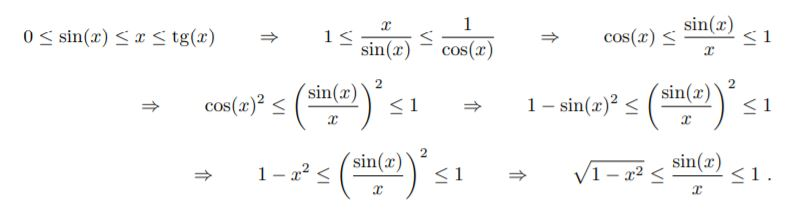
\includegraphics[scale = 0.9]{epflLectureNotes/analysis/figures/usefula.JPG}
    \caption{Useful inequalities}
    \label{fig1}
\end{figure}

\begin{figure}[H]
    \centering
    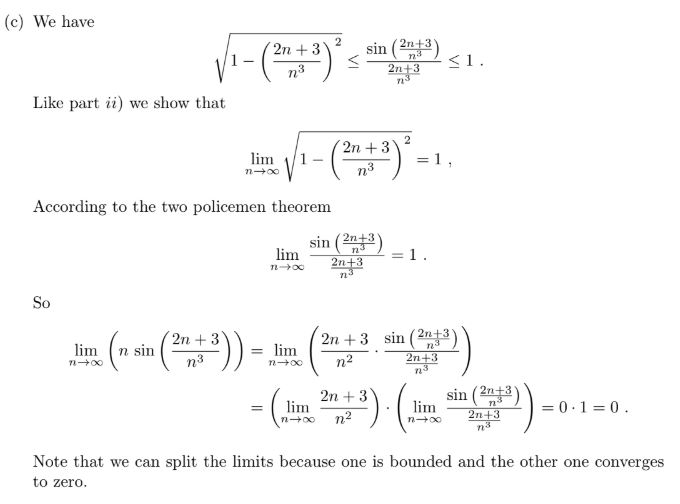
\includegraphics{epflLectureNotes/analysis/figures/usefula2.JPG}
    \caption{Solution to hard limit problem}
    \label{fig2}
\end{figure}

\subsection{More on sequences}
Suppose we want to show that some geometric sequence does not have a limit, simply that it is not converging.

We first establish the \textit{Bernoulli inequality} which we shall prove later. We will use this result immediately. 

\begin{equation}
    q^n \geq 1 + n(q-1)
\end{equation}

\begin{tcolorbox}
Take $x_{n} = 4^n$. Now we claim that $x_{n}$ is not bounded.
\begin{proof}
It is not bounded if we can show that it increasing in increments that do not decrease. Suppose now that $b$ is some upper bound to $x_{n}$. Now by Bernoulli, we have that $4^n \geq 1 + n^\cdot3$. If we can show that $4^n \geq 1 + n\cdot3 > b$ we indeed get that there can be no upper bound $b$. We have that $n > \frac{b-1}{3}$ and such an $\n \in \mathbb{N}$ exists if we set it to $n:= [\frac{b-1}{3} + 1]$ Now since $4^n \geq 1 + n\cdot3$ we have that $x_{n}$ is not bounded. 

\end{proof}
\end{tcolorbox}

\begin{theorem}
Every converging sequence is bounded(a lower or upper bound exists obviously and if convergent the latter also exists.)
\end{theorem}

\clearpage

Let's now get on to proving the rules we established for limit arithmetic.

\begin{proof}(Proof to sum rule)
Now we are given that $x_{n}$ converges to $x$ and that $y_{n}$ converges to $y$. We want to show that $x_{n} + y_{n}$ converges to $x+y$. By definition, this is true if we can show that 
\begin{equation*}
    |(x_{n} + y_{n}) - (x+y)| \leq \epsilon, \ \forall \epsilon \in \mathbb{R}
\end{equation*}

Now luckily we have that $|(x_{y} + y_{n}) - (x+y)| = |(x_{n} - x) + (y_{n} - y)|$ And by the triangle inequality we know that $|(x_{n} - x) + (y_{n} - y)| \leq |x_{n}-x| + |y_{n} - y|$ Thus if we can show that $|x_{n}-x| + |y_{n} - y| < \epsilon$ we are guaranteed that $|(x_{n} - x) + (y_{n} - y)| < \epsilon$ We will succeed with the latter part if we can show that both parts $(x_{n} - x)$ and $(y_{n} - y)$ are smaller than $\frac{\epsilon}{2}$. Now we have by definition of convergence that:

$$ \exists n \geq n_{\frac{\epsilon}{2}}^{x} \rightarrow |x_{n} - x| \leq \frac{\epsilon}{2}$$
Similarly:

$$ \exists n \geq n_{\frac{\epsilon}{2}}^{y} \rightarrow |y_{n} - y| \leq \frac{\epsilon}{2}$$
Now fixing $n_{\epsilon} := \max{n_{\frac{\epsilon}{2}}^{x}, n_{\frac{\epsilon}{2}}^{y}}$(we do this since it assures both conditions to hold we have that because each of $(x_{n} - x)$ and $(y_{n} - x)$ are smaller than $\epsilon$, so must $|x_{n}-x| + |y_{n} - y|$ by the triangle inequality. 
\end{proof}


Let's now do more applications of the squeeze theorem to show limits. 
\begin{example}
We want to show that $aq^{n}$ converges to $0$ for $a\not = 0$ and $|q|<1$. Now as a property we use that $\lim_{n\to\infty}{x_{n}} = 0 \rightarrow \lim_{n\to\infty}{|x_{n}|}=0$ It is clear that we have an inequality of the form $0\leq|aq^{n}|\leq ?$ Doing more algebra(our goal is to find another sequence of form $\frac{1}{x}$ converging to 0 to get:

$$ \frac{1}{?} \leq \frac{1}{|a\cdot q^n|} = \frac{1}{|a|} \cdot (\frac{1}{|q|})^n$$

Now using Bernoulli we have:

$$(\frac{1}{|q|})^n \geq 1 + n(\frac{1}{|q|}-1)$$ which happily means:

$$(\frac{1}{a}\cdot\frac{1}{|q|})^n \geq (\frac{1}{a}\cdot(1 + n(\frac{1}{|q|}-1))$$ 
And finally taking the reciprocal all to get back to $aq^n$ we are left with 

$$ 0 \leq |aq^n| \leq \frac{1}{\frac{1}{a}\cdot(1+n(\frac{1}{|q|}-1)}$$ and clearly we see that the RHS is also a sequence that converges to 0 since all terms in the denominator but $n$ are constants. Hence, we have \textbf{squeezed} our sequence. The key here was that we found a RHS sequence which we wanted to be of form $\frac{1}{x}$ And in addition, we took the reciprocal of the inequality at the start simply to be able to use the bernoulli inequality. 
\end{example}

Let's now consider a harder example.

\begin{example}
Consider the sequence $x_{n} = \sqrt[n]{n}$ Now is this sequence converging? Well we know that $1\leq\sqrt[n]{n}$ and now another sequence we know which approaches to 1 is $1 + \frac{1}{\sqrt{n}}$. Now we only need to show that:

$$\sqrt[n]{n} \leq 1 + \frac{1}{\sqrt{n}} $$ holds and if we can show this, we'll have that our sequence converges to 1. 

Now we get:
$$ n \leq (1 + \frac{1}{\sqrt{n}})^n$$ And notice how $(1 + \frac{1}{\sqrt{n}})^n$ is simply a binomial hence if any one of the terms in the binomial expansion is greater than $n$ our inequality will hold(this works as all $n$ are positive). Well for $\sum_{i=0}^{n}{n\choose i}(\frac{1}{\sqrt{n})^{i}}$ when observe that for $i=4$ we get:

$$\frac{(n-1)(n-2)(n-3)}{24n} \geq n$$ further reducing to:
$$\frac{24n^2}{(n-1)(n-2)(n-3)} \leq 1$$ and we know this is valid as 

$$\lim_{n\to\infty}{\frac{24n^2}{(n-1)(n-2)(n-3)}} = 0$$
 
Hence we get that $$\sqrt[n]{n} \leq 1 + \frac{1}{\sqrt{n}} $$ meaning that $\sqrt[n]{n}$ converges to 1. 
\end{example}

Let's do one last example:

\begin{example}
Consider $x_{n} = \frac{2^n}{x!}$ Now clearly $0\leq\frac{2^n}{x!}$ and observing that $\frac{2^n}{x!} = \frac{2}{1} \cdot \frac{2}{2} \cdot \frac{2}{3} \ldots $ it is obvious that $\frac{2^n}{x!} \leq 2 \cdot (\frac{2}{3})^{n-2}$ But we know that $\lim_{n\to\infty}{2 \cdot (\frac{2}{3})^{n-2}}=0$ hence we have again squeezed our sequence!
\end{example}

\begin{theorem}
If $\lim_{n\to\infty}{x_{n}}=0$ and $y_{n}$ is bounded, then $\lim_{n\to\infty}{x_{n}\cdot y_{n}}=0$
\end{theorem}

\begin{theorem}
\label{monotone}
If a sequence is bounded and increasing(monotone) it converges to the supremum (resp. infimum). 
\end{theorem}

\begin{proof}
Now because $y_{n}$ is bounded, we have that $\exists M$ s.t. $M\geq y_{n} \forall n$. Hence we obtain that $x_{n}y_{n} \leq Mx_{n}$ and clearly since $Mx_{n}$ converges to $0$ we have squeezed $x_{n}y_{n}$ and have that it also converges to 0. 
\end{proof}


We consider the famous sequence of \textbf{Fibonacci quotients}
\\
Now the fibonacci sequence is defined as $x_{0}=x_{1} = 1$, $x_{n+1} = x_{n} + x_{n-1}$ and we define the sequence of fibonacci quotients as $y_{n} = \frac{x_{n+1}}{x_{n}}$ Our first theorem is that fibonacci quotient sequence is bounded between 1 and 2. Let's now fnd it's limit. Notice firstly that $y_{n+1} = 1 + \frac{1}{y_{n}}$
    $$y = \lim_{n \to \infty}{y_{n}} = \lim_{n \to \infty}{y_{n+1}} = 1 + \frac{1}{\lim_{n\to \infty}{y_{n}}} $$ Hence we get:
    
    $$ y = 1 + \frac{1}{y}$$ which gives $\frac{1+\sqrt{5}}{2}$ as the only valid solution. But we still have to show that our sequence converges. A smart way to do so is to show that $z_{n} := |y_{n} - \frac{1+\sqrt{5}}{2}|$ converges which by limit arithmetic would imply $\lim_{n \to \infty}{y_{n}} = \frac{1+\sqrt{5}}{2}$ Our goal is to squeeze $z_{n}$ in doing so. Notice that $z_{n+1} = |y_{n+1} - \frac{1+\sqrt{5}}{2}|= \underbrace{1 + \frac{1}{y_{n}} - (1 + \frac{2}{1+\sqrt{5}})}_{\text{ using definition }} $ This yields the inequality $z_{n + 1} = \frac{|y_{n} - \frac{1+\sqrt{5}}{2}|}{y_{n}\frac{1+\sqrt{5}}{2}}= \frac{2}{1+\sqrt{5}}\frac{|y_{n - \frac{1+\sqrt{5}}{2}}|}{y_{n}}$ to give us that $z_{n+1} \leq \frac{2}{1+\sqrt{5}}|y_{n - \frac{1+\sqrt{5}}{2}}|}$ because we know that $y_{n} \geq 1$. Now finally this simplifies to $z_{n+1} \leq \frac{2}{1+\sqrt{5}}z_{n}$ which applying the definition of $z_{n}$ gives $z_{n} \leq \frac{2}{1+\sqrt{5}}^{2}z_{n-1} $ to result in $z_{n} \leq \frac{2}{1+\sqrt{5}}^{n}z_{0}$ which converges to 0. Hence we have squeezed $z_{n}$
    
    \clearpage
    
    In general this is the scheme one should use for finding limits of recursive sequences:
    
     \begin{tcolorbox}[drop shadow, title = (Limit of recursive sequence),lower separated=true]
     \begin{enumerate}
         \item Assuming there is a limit, compute it using limit algebra.
         \item Showing some upper and lower bound(using induction) exclude any extra answers.
         \item Finally show that the sequence converges by showing that $\lim_{n\to\infty}{x_{n}-x}=0$
     \end{enumerate}
\end{tcolorbox}

We now come to define \textbf{approaching infinities}.
\begin{definition}
The definition of approaching $\infty$ is as intuitive as saying for any real number I pick, the sequence has a term larger than it. Hence we define $\lim_{n\to \infty}{x_{n}} = \infty$ as $\forall A \in \mathbb{R}$ $\exists n_{A} \in \mathbb{N}$ such that $n\geq n_{A}$ and $x_{n} \geq A$. The similar definition applies for approaching $-\infty$
\end{definition}

\begin{example}
Notice that for a geometric sequence $x_{n} = aq^{n}$ if $a>0$ and $q>1$ it approaches $\infty$ and if $a<0$ and $q>1$ it approaches $-\infty$ 
\end{example}

A set of useful theorems on approaching infinities is the following:

\begin{theorem}(Theorems on approaching infinity)
\\
If $\lim_{n\to\infty}{x_{n}} = \infty$ and $y_{n}$ is bounded from below, then $\lim_{n\to\infty}{x_{n} + y_{n}} = \infty$
\\
If $x_{n}$ and $y_{n}$ both approach infinity, so does their product.
\\
If $y_{n}$ is bounded and $x_{n}$ approaches infinity, then $\lim_{n\to\infty}{\frac{y_{n}}{x_{n}}} = 0$
\end{theorem}

We note that when it is the case that $\lim_{n\to\infty}{x_{n}}=\infty$ and  $\lim_{n\to\infty}{x_{n}}=-\infty$ we may have different cases such as:

$$ \lim_{n\to\infty}\underbrace{n}_{x_{n}} + \underbrace{(-n)}_{y_{n}} = 0 $$

$$\lim_{n\to\infty}\underbrace{2n}_{x_{n}} + \underbrace{(-n)}_{y_{n}} = \infty$$

$$\lim_{n\to\infty}\underbrace{2n + (-1)^{n}n}_{x_{n}} + \underbrace{(-2n)}_{y_{n}} = (-1)^{n}n \text{ which is unbounded hence does not approach anything}$$


\begin{theorem}(Squeeze theorem for approaching infinities)
For sequences $x_{n}$ and $y_{n}$ if $\exists n_{0} \in \mathbb{N}$ such that $\forall n \geq n_{0}$, $x_{n} \leq y_{n}$ we have:
\\
(1) If $\lim_{n\to\infty}{x_{n}} = \infty$ then $\lim_{n\to\infty}{y_{n}} = \infty$
\\
(2) If $\lim_{n\to\infty}{y_{n}} = -\infty$ then $\lim_{n\to\infty}{x_{n}} = -\infty$
\end{theorem}

\begin{theorem}(Quotient criterion)
\\
$\forall x_{n} \not = 0$ and $\lim_{n\to \infty}{|\frac{x_{n+1}}{x_{n}}|} = \infty$ then we have that $x_{n}$ diverges. 
\end{theorem}

And now we provide an example of sandwich for infinities. 

\begin{example}
Define $x_{n}:= \frac{x!}{2^{n}}$ We have that $\frac{n}{2} \cdot \frac{n-1}{2} \ldots \cdot \frac{3}{2} \ldots \geq \frac{n}{2} \cdot \frac{3}{2}^{q-1}$ for some $n$. And because the latter is a geometric sequence which noticeably approaches infinity we have that $x_{n}$ approaches infinity. 
\end{example}

\begin{proof}(We present a proof to theorem \ref{monotone})
\\
Now set $S:=sup\{x_{n}|n\in\mathbb{N}\}$ and let $0<\epsilon\in\mathbb{R}$ By definition $S$ is the smallest bound hence $S-\epsilon$ is not the smallest bound. By def. again, $\exists n_{\epsilon}$ such that $S-\epsilon<x_{n_{\epsilon}}$ and we now get (for $n\geq n_{\epsilon}$ 
$$S - \epsilon < x_{n_{\epsilon}} < x_{n} < S < S+\epsilon$$ and this is exactly the definition of convergence hence $S$ is the limit.
\end{proof}
\clearpage

     \begin{tcolorbox}[drop shadow, title = (Exploration of e),lower separated=true]
   We define $x_{n} = (1 + \frac{1}{n})^n$ We first ask is $x_{n}$ increasing. Consider the claim $(1+\frac{1}{n})^{n} < (1+\frac{1}{n+1})^{n+1}$
   Now let's consider both the expansions of $(1 + \frac{1}{n})^n$ and of $(1 + \frac{1}{n+1})^{n+1}$
   
   $$ (1 + \frac{1}{n})^n = \sum_{i=0}^{n} \binom{n}{i} (\frac{1}{n^n}) = \sum_{i=0}^{n} \frac{1}{i!} \frac{n\cdot (n-1) \ldots (n-i+1)}{n^i} = \sum_{i=0}^{n} \frac{1}{i!} (1 - \frac{1}{n}) \ldots (1 - \frac{i-1}{n})    $$
   
   Similarly we have:
   $$ (1 + \frac{1}{n + 1})^{n+1} = \sum_{i=0}^{n} \frac{1}{i!} (1-\frac{1}{n+1}) \ldots  (1 - \frac{i-1}{n}) $$
   
   and because generally $\frac{
   q}{j} > \frac{q}{j+1}$ we have that terms on the RHS of the first expression are larger hence $(1+\frac{1}{n})^{n} < (1+\frac{1}{n+1})^{n+1}$ And we also have that our sequence is less than 3(which we do not show).
   
   Thus we define $$\lim_{x \to \infty}{(1+\frac{1}{n})^{n}} = e$$
\end{tcolorbox}

And now we present an example of a bounded sequence that is decreasing which converges to its infimum. Consider $x_{n+1} = \frac{1}{2}(x_{n} + \frac{1}{x_{2}})s$ and $x_{0}= 2$.
\\
We claim 1 is a lower bound which is true by induction(easy to show). Similarly, the sequence is decreasing as $x_{n} - x_{n+1} = \frac{1}{2}(x_{n}-\frac{1}{x_{2}} \geq 0$ since $x_{n} \geq 1$ And applying the recursive formula as usual we find that the limit is either -1 or 1 and ruling out -1 we get 1.  

\subsection{More definitions and theorems}

We come to an interesting definition. That of \textit{LimSup & LimInf}.

\begin{definition}(LimSup and LimInf)
Let $x_{n}$ be a bounded sequence. Then:
$$y_{n} := \sup{\{x_{k}|n\leq k \in \mathbb{N}\}} \text{(resp. inf)}}$$
\end{definition}

Now the sequence $y_{n}$ is clearly decreasing as we are looking over a smaller set for each $n+1$. Similarly considering the respective inf definition, we have that it is increasing as each time we are removing elements from the largest set for $n=0$ meaning that our inf is at least as large as $y_{0}$ or bigger. Now since $y_{n}$ is valid sequence definition, it naturally has a limit as well defined as:

$$y_{n} := \lim_{n\to\infty}{\sup{\{x_{k}|n \leq k \in \mathbb{N}\}} \text{(resp. inf)}}}$$


\begin{remark}
       The purpose in defining limsup and liminf is that when a limit on itself doesn't exist, by taking limsup, we limit the values of our sequence and if for instance our sequence consists of purely -1 and 1 limsup tells us that the largest occurring value is 1. In the case where our sequence approached $\infty$ so does limsup and whenever a limit exists, limsup is the limit. 
\end{remark}

Here's an example:

\begin{example}
Consider $x_{n} = (-1)^{n}$. Defining $y_{n} = \sup{\{x_{k}|n\leq k \in \mathbb{N}\}}$ we get that the limit of $y_{n}$ as n goes to infinity is 1. 
\end{example}

And now we define what it means to be a subsequence. 

\begin{definition}
Let $x_{n}$ be a sequence. Then $x_{n_{k}}$ is a subsequence of $x_{n}$ where each $k$ is mapped to some $n_{k}$ by some rule $f: \mathbb{N} \to \mathbb{N}$
\end{definition}

\begin{example}
Suppose we define $x_{n} = \frac{1}{n}\sin{n}$ And define the subsequence $x_{2\pi k}$ we notice that this subsequence is constant with all values mapping to $0$
\end{example}

And yet a meatier example is:

\begin{example}
Define $x_{n} = (1 + \frac{2}{n})^{n}$ and a subsequence $x_{2k}$. We notice that 
$$ \lim_{k \to \infty}{(1 + \frac{1}{k})^{2k}} = \lim_{k \to \infty}{(1 + \frac{1}{k})^{k})^{2}} = e^{2}$$
\end{example}


\begin{theorem}
If a sequence $x_{n}$ converges to $a$, then so do all subsequences of $x_{n}$
\end{theorem}

\begin{proof}(Simply using invoking definition of convergence)
Now accepting the if true, we have that:

$$ \forall \epsilon > 0, \ \exists n_{\epsilon} \ \text{s.t.} n\geq n_{\epsilon} \rightarrow |x_{n} - a| \leq \epsilon$$

\textcolor{red}{We now fix $n_{\epsilon} = n_{k}$ hence proof. (this proof is to be revisited, it may be false.}
\end{proof}

\begin{example}
Consider a sequence that jumps between $e$ and $-e$ as $n \to \infty$ defined by $x_{n} = (-1)^{n}(1 + \frac{1}{n})^{n}$ For all subsequences with an even domain, the limit is $e$ and for subssequences with an odd domain, limit is $-e$
\end{example}

\begin{theorem}(Bolzano Weierstrass)
Every bounded sequence contains a convergent subsequence. 
\end{theorem}

\begin{proof}
Let's define $y_{n} = \sup{x_{k}:k\geq n}$. Now given that $y_{n}$ is bounded from below(because $x_{n}$ is bounded) and that it is decreasing, we have that $y_{n}$ converges to some $y$ meaning:
$$ \forall \epsilon > 0, \forall N, \exists n_{\epsilon} \geq N \ , \underbrace{|y_{n} - y|\leq \frac{1}{2}\epsilon}_{\text{definition of convergence}}$$

And by definition of sup and how we defined $y_{n}$ we have that 
$$ \forall \epsilon > 0, \exists n_{1} \geq n \rightarrow |x_{n_{1}} - y_{n}| \leq \frac{1}{2}\epsilon$$

Considering that we want an expression like $|x_{n_{1}} - y|\leq\epsilon$ And we get this by:

$$ |x_{n_{1}} - y| = |x_{n_{1}} - y_{n} + y_{n} - y| \leq \underbrace{|x_{n_{1}} - y_{n}| + |y_{n} - y_{n}|}_{\text{using triangle ineq.}} \leq \frac{1}{2}\epsilon + \frac{1}{2}\epsilon = \epsilon $$
Now the last part is enough for the proof because we are assured that for any subsequence choice we make, it holds that there is an $N$ such that $n_{k} \geq N$
\end{proof}


\begin{definition} (Cauchy convergence)
A sequence is Cauchy convergent if $\forall \epsilon > 0$, $\exists n_{\epsilon}$ such that $\forall n,m \geq n_{\epsilon}$ we have that $|x_{n} - x_{m}| \leq \epsilon$
\end{definition}

A very important theorem concerning Cauchy convergence is:


\section{Series}

\begin{definition}
A series $S_{n}$ is defined in terms of the summation of some sequence $x_{n}$.

$$S_{n} = \sum_{k=0}^{n} x_{n}$$
\end{definition}

\begin{theorem}(Bernoulli Inequality(Known as the negative case of it)
\\
Whenever $-1<x<0$ we have that $(1+x)^{n} \geq 1 + nx$
\end{theorem}
\\

\begin{definition}(Cauchy criterion for series)
A series $S_{n}$ is convergent iff: 
$$ \forall \epsilon >0, \exists n_{\epsilon} \ \forall n,m > n_{epsilon} \ \sum_{k = n+1}^{m} |x_{k}| \leq \epsilon$$
\end{definition}

\begin{theorem}
As follows from the Cauchy criterion, we have that  $\forall \epsilon >0, \exists n_{\epsilon} \ \forall n,m > n_{epsilon} \ \sum_{k = n+1}^{m} |x_{k}| \leq \epsilon$ which means that if we let $m=n+1$ we obtain $|x_{n+1}|\leq \epsilon$ which by definition of the limit says that $x_{n+1}$ goes to 0. 
\end{theorem}


     \begin{tcolorbox}[drop shadow, title = (Yet another way to obtain e),lower separated=true]
     Consider the sequence $S_{n} = \sum_{k=0}^{\infty} \frac{1}{k!}$
     Now clearly $S_{n}$ is increasing and is bounded. It is bounded because:
     
     $$\sum_{k=0}^{\infty} \frac{1}{k!} \leq 1 + \sum_{k=1}^{n} \frac{1}{2^{k-1}} \leq 1 + \sum_{k=1}^{\infty} \frac{1}{2^{k-1}} = 3$$
     
     Thus we know that a limit must exists. Now let's find that limit. Observe that:
     
     $$\sum_{k=0}^{\infty} \frac{1}{k!} \geq \sum_{k=0}^{\infty} \frac{1}{k!}\underbrace{(1 - \frac{1}{n}) \ldots (1 - \frac{k-1}{n})}_{\text{each term smaller than 1}} \geq 2 + \sum_{k=2}^{\infty} \frac{1}{k!}\underbrace{(1 - \frac{1}{n}) \ldots (1 - \frac{k-1}{n})}_{\text{first 2 terms are 1}}$$
     
     And further realizing that:
     
      $$2 + \sum_{k=2}^{\infty} \frac{1}{k!}(1 - \frac{1}{n}) \ldots (1 - \frac{k-1}{n})} \geq 2 + \sum_{k=2}^{\infty} \frac{1}{k!}(1 - \frac{k-1}{n}^{k-1})} \geq \sum_{k=0}^{n} \frac{1}{k!}\underbrace{(1 - \frac{k-1}{n}(k-1))}_{\text{\makebox[0pt]{Using negative Bernoulli}}} $$
      
      Now the very last term on the RHS is equal to: 
      
      $$ \sum_{k=0}^{n} \frac{1}{k!} - \frac{1}{n}\sum_{k=2}^{n} (\frac{(k-1)^2}{k!}$$
      
      Now we are in a very good position because we have that 
     
     $$\sum_{k=0}^{\infty} \frac{1}{k!} \geq \sum_{k=0}^{\infty} \frac{1}{k!}(1 - \frac{1}{n}) \ldots (1 - \frac{k-1}{n}) \geq  \sum_{k=0}^{n} \frac{1}{k!} - \frac{1}{n}\sum_{k=2}^{n} (\frac{(k-1)^2}{k!}$$
     
     Which means that if we can show that $\frac{1}{n}\sum_{k=2}^{n} (\frac{(k-1)^2}{k!})$ tends to 0 and given that $\sum_{k=0}^{\infty} \frac{1}{k!}(1 - \frac{1}{n}) \ldots (1 - \frac{k-1}{n}) \to e$ we will have squeezed $e$ between $\sum_{k=0}^{n} (\frac{1}{k!})$
     
     Now notice that:
     $$\frac{1}{n} \to 0 , \frac{1}{n}\sum_{k=2}^{n} (\frac{(k-1)^2}{k!} \leq \frac{1}{n}\sum_{k=2}^{n} \frac{1}{(k-2)!}} = \frac{1}{n}\sum_{k=0}^{n-2} \frac{1}{(k)!}}  \leq 3$$
     
     Thus we gloriously obtain that :
     $$ \sum_{k=0}^{n} \frac{1}{k!} \geq e \geq \sum_{k=0}^{n} \frac{1}{k!}$$
    
\end{tcolorbox}

\clearpage

\begin{definition}
A series is convergent if simply $S_{n}$ is convergent and it is absolute convergent if $S_{n} = \sum_{k=0}^{n} |x_{k}|$ is convergent.
\end{definition}

Now a very important theorem is the following:

\begin{theorem}
If $\sum_{k=0}^{n=\infty}x_{k}$ is convergent, then $\lim_{n\to\infty}x_{n} = 0$
\end{theorem}

And squeeze theorem for series is;

\begin{theorem}
assume $\exists n_{0}$ s.t. $0\leq x_{n} \leq y_{n} \ \forall n \geq n_{0}$ Then: 
\begin{enumerate}
    \item if $\sum_{k=0}^{\infty} y_{k}$ is convergent, so is $\sum_{k=0}^{\infty} x_{k}$
    \item if $\sum_{k=0}^{\infty} x_{k}$ is divergent, so is $\sum_{k=0}^{\infty} y_{k}$
\end{enumerate}
\end{theorem}

And more theorems:

\begin{theorem}
Whenever $x_{k} \geq 0$ a series is:
\\
\begin{empheq}[left =\text{$\sum_{k=0}^{\infty} x_{k}$}\empheqlbrace]{align*}
\text{Convergent if $S_{n}$ is bounded.} \\
\text{Divergent else.}
\end{empheq}
\end{theorem}

And now we define a \textbf{Leibniz series} as being of form $S_{n} = \sum_{k=0}^{n} (-1)^{k}(x_{k})$ And the important Leibniz criterion is:

\begin{theorem}
For a Leibniz $S_{n}$, $S_{n}$ diverges if $x_{k}$ is decreasing and $\lim_{n\to\infty}(x_{n}) = 0$
\end{theorem}

\begin{prop}
If $S_{n}$ is absolute convergent, then it is convergent. 
\end{prop}

The above is obvious to see using Cauchy criterion. Now absolute convergence implies:

$$ \sum_{k=n+1}^{m} |x_{k}| \leq \epsilon$$ and the triangle inequality gives us that $$ |\sum_{k=n+1}^{m} x_{k}| \leq \sum_{k=n+1}^{m} |x_{k}| $$ hence we know that $$  |\sum_{k=n+1}^{m} x_{k}| \leq \epsilon$$ which is exactly what we want. 
And the last thing we do on series is to present the Cauchy and Alembert convergence criteria:

\begin{figure}[H]
    \centering
    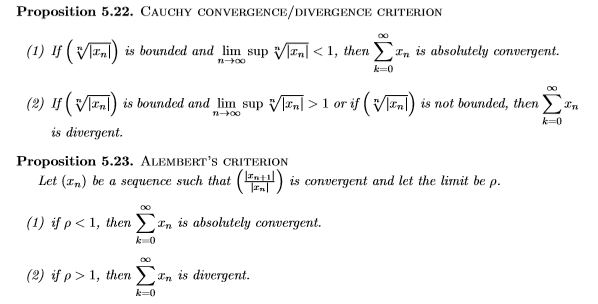
\includegraphics{epflLectureNotes/analysis/figures/series.JPG}
    \caption{Yes I was lazy to write this down}
    \label{fig:my_label}
\end{figure}

\begin{theorem}
Yet another important fact is that the harmonic series defined in terms of summing $\frac{1}{n}$ diverge(one would have expected) it to converge.
\end{theorem}

And another important and rather obvious theorem is:

\begin{theorem}
Whenever a sequence maps $\mathbb{N} \to \mathbb{R^{+}}$ or the opposite and all of its partial sums are bounded, then the series converges.
\end{theorem}

\section{Real-valued functions of 1-variable}
\subsection{Basics}
\begin{definition}(Defining what it means to be  a function of one variable)
\\
Let $E\subseteq\mathbb{R}$. Then $f$ is subset of $E\times\mathbb{R}$ where each element of $f$ is of form $(a,b)$ and each $a$ occurs only once. 
\end{definition}
\\

Something taught at high-school is the local maximum. We now formally define it:

\begin{definition}(Local maximum)
Some $f:E\to\mathbb{R}$ has a local maximum at $x_{0}$ if $\forall \sigma > 0$, $\exists x$ such that $|x_{0} - x| < \sigma \rightarrow f(x_{0}) > f(x)$
\end{definition}
\\

We say that some $f:E\to\mathbb{R}$ is defined a pointed neighbourhood of $x_{0} \in \mathbb{R}$ if $\exists$ an interval $]x_{0}-a,x_{0}+a[$ contained in $E\backslash\{x_{0}\}$
\\

We now define what it means to be the limit of a function. 

\begin{definition}
Suppose $f:E\to\mathbb{R}$ is defined on a pointed neighbourhood of $x_{n}\in \mathbb{R}$. We say that $\lim_{x \to x_{0}} f(x) = L$ if:
\begin{enumerate}
    \item $\forall 0 < \epsilon \in \mathbb{R}$, $\exists 0<\sigma \in \mathbb{R} $ such that $|x - x_{0}| < \sigma \rightarrow |f(x) - L| < \epsilon$
    \item for every sequence $x_{n} \subseteq E-\{x_{0}\}$ we have that $\lim_{n\to \infty}x_{n} = x_{0} \rightarrow \lim_{n\to\infty}f(x_{n})= f(x_{0}) = L$
\end{enumerate}
\end{definition}

\begin{example}
Let's show that $\lim_{x\to 2}(x^2) = 4$ using the first definition.
We need:
$$ |x-2| < \sigma \rightarrow |x^2 - 4| < \epsilon$$
Now pick suppose that $|x-2| \leq 1 $ which yields that $ 1\leq x \leq 3 \equiv 3\leq x + 2 \leq 5$ Particularly because $|x+2| \leq 5$ we get that:
$$ |x-2||x+2| = |x^2 - 4| \leq 5|x-2|$$
Now finally set $\sigma := \min{1,\frac{\epsilon}{5}}$ because then if:
$$ |x-2| \leq 1 \ \text{and} \ |x-2| \leq \frac{\epsilon}{5}$$ we get that:
$$ |x^2 - 4| \leq \underbrace{5|x-2|}_{\text{\makebox[0pt]{because $|x+2|\leq5$}}} \leq 5\frac{\epsilon}{5}$$
\end{example}
  
Let's now go through an example demonstration using the sequence definition of the limit.

\begin{example}
Suppose we want to show that for $f(x) = x^2 + 1$ $ \lim_{x \to 0} x^2 + 1 = 1$. Now define $x_{n} = n$ which gives us a sequence such that $\lim_{n \to \infty}x_{n} = 0$. Now we want $\lim_{n \to \infty}x_{n}^{2} + 1 = 1$. By limit algebra we get:
$$ = (\lim_{n \to \infty}x_{n})^2 + 1 = 0^2 + 1 = 1$$
\end{example}

\begin{definition}
some $f$ is continuous in $x_{0}$ if $\lim_{x \to x_{0}} f(x)$ exists and is equal to $f(x_{0})$ which extrapolates to, $f:E \to \mathbb{R}$ is continuous if it is continuous $\forall x \in E$
\end{definition}

And now let's take the example of a function for which a limit does not exists. 

\begin{example}
Suppose $f$ is given by:

$$ \begin{empheq}[left =\text{$f(x) = $}\empheqlbrace]{align*}
\text{1 if $x \in \mathbb{Q}$} \\
\text{0 if $x \in \mathbb{R}\backslash \mathbb{Q}$}
\end{empheq}$$

Now notice that we can pick $\lim_{n \to \infty}\frac{1}{n} = 0$ and $\lim_{n \to \infty}\frac{\sqrt{2}}{n} = 0$ but we have that the latter has limit $1$ and the former limit $0$. 
\end{example}
\\
And now using our earlier construct of the limit of a function, we define what it means for $f$ to be continuous at $x_{0}$
\\

$f(x)$ is continuous at $x_{0}$ if $\lim_{x\to x_{0}} f(x) = f(x_{0})$ And in general, $f$ is \textbf{continuous} if it is continuous $\forall x \in \mathbb{R}$

And now let's show that $sin(1/x)$ is not continuous at $0$.

\begin{example}
define $x_{n} := \frac{1}{\pi(2n+\frac{1}{2})}$ and $y_{n} := \frac{1}{\pi(2n+\frac{3}{2})}$ Now both sequences converge to $0$. Yet we have that $f(x_{n})$ converges to 1 whereas $f(y_{n})$ converges to -1. 
\end{example}
\\

And now we highlight limit algebra for functions. It is all very similar to limit algebra of sequences since the sequence definition tells us that $\lim_{x \to \infty} f(x_{n}) = L$ and supposing also that $\lim_{x \to \infty} g(x_{n}) = k$ we have:

\begin{align*}
    \lim_{x \to \infty}(f + g)(x_{n}) = L + K\\
    \lim_{x \to \infty}(f\cdot g)(x_{n}) = L\cdot K\\
    \lim_{x \to \infty}(\frac{f}{g})(x_{n}) = \frac{L}{K} \ \text{whenever $x \not = 0$}
\end{align*}

And now squeeze for limits of functions:

\begin{theorem}
Suppose that $\lim_{x \to \infty} g(x_{n}) = k$ and that $\lim_{x \to \infty} f(x_{n}) = L$ such that a pointed neighbourhood of some $x_{0}$ is also a subset of the domain of $h(x)$. Now on some neighbourhood of $x_{0}$:
\\
$f(x) \leq h(x) \leq g(x)$\\
$l = k$
\\
then \ $\lim_{x \to \infty}h(x) = l$
\end{theorem}

\begin{example}
Consider $\lim_{x \to 0} \frac{\sin(x)}{x}$. We have that $\frac{\sin(x)}{x} \leq 1$ and also that $\frac{\sin(x)}{x}\geq \cos(x)$ As both approach $1$ so does our function. 
\end{example}

And some more theorems on continuity:
\begin{theorem}
If $f$ and $g$ are continuous functions defined on the same domain, then we have are continuous as well:
\begin{enumerate}
    \item $af + bg \forall a,b \in \mathbb{R}$
    \item $f\cdot g$
    \item $g|_{E}$ (to mean that $\forall x \in E, f(x) \not = 0$) where $\frac{f}{g}$
\end{enumerate}
\end{theorem}

And as for composition of functions, we state the composed map is continuous iff. both functions are continuous and the image of the inside function is a subset of the domain of the outer function.
\\

And now our goal is to define limits at infinity. Let's first define a pointed neighbourhood at infinity:

\begin{definition}
A pointed neighbourhood of $+\infty$ is an open interval of form $]a,+\infty[$
\end{definition}

Now for one last time, let's recall what it means for a function $f:E \to \mathbb{R}$ to have a limit $L$ at some $x_{0}$ We say that $\lim_{x\to x_{0}} f(x) = L$ iff :
$$ \forall (x_{n} \in \mathbb{E}\backslash\{x_{0}\}) \ lim_{n \to \infty}x_{n} = x_{0} \rightarrow \lim_{n \to infty} f(x_{n}) = f(x_{0})$$

\begin{prop}
We claim that $\lim_{x \to 0} \frac{1}{x}$ does not exist. To see this consider $x_{n} = \frac{1}{n}$ defined on $]a,\infty[$ and $y_{n} = \frac{-1}{n}$ defined on $]- \infty, -a[$ Now both sequences are defined on the pointed neighborhood $\mathbb{R}\backslash \{0\}$ yet the first approaches $\infty$ and the latter $- \infty$  
\end{prop}

\begin{tcolorbox}[drop shadow, title = (Limit of functions algebra),lower separated=true]

for functions $f,g: E \to \mathbb{R}$
\begin{enumerate}
    \item (Addition rule)
    \\
    if $f$ approaches infinity at $x_{0}$ and $g$ is bounded from below then: $(f+g)(x)$ approaches infinity at $x_{0}$. 
      \item (Product rule)
    \\
    if $f$ approaches infinity at $x_{0}$ and $g$ is bounded from below by a positive number and $f(x)g(x) > 0 \forall x \in E$ then: $(fg)(x) \to \infty$ at $x_{0}$. 
    \\
    
    \item (First division rule)
    \\
    we have that $f$ is bounded, $g$ is nowhere 0 and $\lim_{x \to x_{0}}|g(x)| = \infty$ then $\lim_{x \to x_{0}} \frac{f(x)}{g(x)} = 0$
    \\
    
    \item (Second division rule)
    \\
    we have that $f$ is bounded from below by a positive number, $g(x)$ converges to 0 at $x_{0}$ and $\frac{f(x)}{g(x)} > 0$ then $\frac{f(x)}{g(x)}$ approaches $+\infty$ at $x_{0}$
    \\
    
    We do not state the squeeze theorem as it is essentially the same as that for non-infinity limits of functions. 
    \\
    
    In particular, a rule of thumb is to never use the addition rule for limits of type $ \infty - \infty$ which is also obvious from how we defined the bounded below property. 
\end{enumerate}
\\
\end{tcolorbox}

Now how do we make sense of limits for which a left or a right side does not exists aka.(a pointed neighbourhood of some $x_{0}$ is not a subset of the domain. We introduce left and right neighbourhoods. 

\begin{definition}
A left neighbourhood(voisinage a gauche in French) of $x_{0}$ is a closed interval of the form $]x_{0} - \delta, x_{0}[$ (resp. applies right neighbourhood)
\end{definition}
\\

Using this we define limits from the right and from the left denoted by $x_{0}^{+}$ and $x_{0}^{-}$
\\

\begin{example}
$\lim_{x\to 0^{+}} \sqrt{x} = 0$ since this definition invokes a right neighbourhood of $x_{0} = 0$. 
\end{example}
\\

Now an important theorem following from this is the following:

\begin{theorem}
If the right and left limit of $f$ at $x_{0}$ are equal, then $f$ is said to \textit{have a limit at $x_{0}$}
\end{theorem}

\begin{figure}[H]
    \centering
    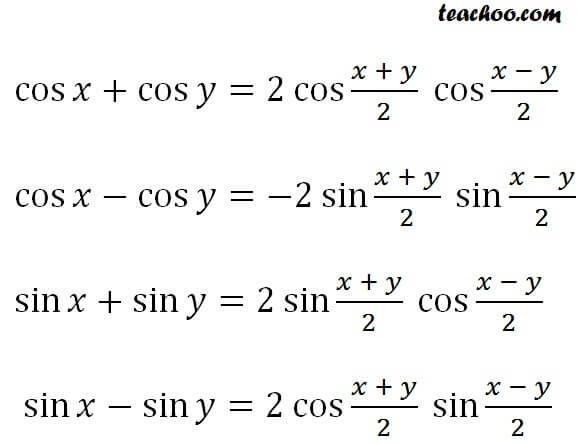
\includegraphics[scale = 0.3]{epflLectureNotes/analysis/figures/formula.jpg}
    \caption{Your friend for exams}
    \label{fig:my_label}
\end{figure}

\subsection{More continuity and consequences}

We remind once again that a function is said to be continuous iff it is continuous forall $x$ in its domain. That is, both $\frac{1}{x}$ and $\frac{1}{x^{2}}$ are continuous on $\mathbb{R}\backslash\{0\}$. Similarly any $p \in \mathbb{P}_{n}$ is continuous over $\mathbb{R}$
\\

When it comes to some monotone sequence approaching infinity, if the sequences is bounded it's limit simply becomes the sup of its image. Otherwise we say that it tends to infinity. 
\\

And now uniform continuity:
\begin{theorem}
A function $f:E \to \mathbb{R}$ is uniformly continuous iff. $\forall \epsilon > 0$, $\exists \delta > 0$ s.t. $\forall x,y \in E$ we have:
$$|x-y| < \delta \rightarrow |f(x) - f(y)|<\epsilon$$
\end{theorem}
Note that this definition differs from continuity in that it states for all $x,y$ whereas in continuity we state that for a given $x_{0}$. 
\\

\begin{tcolorbox}
\begin{remark}
       Speaking in a naive sense, continuity is to say that a small change in x results in a small change in its image. However as we move across the domain, this small change in x may gradually cause a larger and larger increase between two near x's. However uniform continuity asserts that the small change in the image of our x is uniform aka. constant. 
\end{remark}
\end{tcolorbox}

\begin{theorem}
Uniform continuity implies continuity. 
\end{theorem}

\begin{example}
$f(x) = x^2$ is not uniformly continuous. To show this, we need the negation of implication which is $|x-y|<\delta$ and $|x^{2} - y^{2}|\not<\epsilon$ Now set $|x+y|>\frac{2\epsilon}{\delta}$ and $|x-y| = \frac{\delta}{2}$ hence simply pick to very large numbers that are very close to each other. But then because $|x^2 - y^2| = |x-y||x+y| \geq \frac{2\epsilon}{\delta}\frac{\delta}{2} = \epsilon$ hence a contradiction. 
\end{example}

\begin{prop}
$\cos{x}$ is uniformly continuous hence also continuous.
\end{prop}

\begin{proof}
Now we have that $|\cos{x} - \cos{y}|=2|\sin{\frac{x+y}{2}}\sin{\frac{x-y}{2}}| \leq 2|\sin{\frac{x+y}{2}}|\leq 2|x-y|$

And now we have that:(setting $\delta = \frac{\epsilon}{2}$
$$|x-y|\leq \delta \rightarrow |\cos{x} - \cos{y}|\leq  2|x-y|\leq \epsilon$$
\end{proof}


\begin{remark}\textbf{Difference between uniform and standard continuity}
\\
The only difference between the two definitions is the order of quantifiers. That is, $f$ is continuous on $A$ if:
$$\forall c \in A \ \forall \epsilon > 0 \ \exists \delta > 0 \ \forall x \in \ A[ |x-c| \leq \delta \rightarrow |f(x) - f(c)|\leq \epsilon|$$ Whereas $f$ is uniformly continuous on $A$ if: 
$$\forall \epsilon > 0 \ \exists \ \delta > 0 \ \forall x,c \in A \ [|x-c| \leq \delta \rightarrow |f(x) - f(c)|\leq \epsilon|]$$

This goes on to simply show that in uniform continuity, our choice of $\delta$ is independent of the value of $c$. So if we imagine our chosen epsilon and delta as forming a rectangle, then uniform continuity implies that there is always a delta value such that the rectangle may be fitted in any arbitrary range in the domain. This also then clarifies why uniform continuity implies contunuity. 
\end{remark}

\begin{example}\textbf{(Continuous extensions)}
\\
Consider $f:]0,1]\backslash A \to \mathbb{R}$ where $A = \{(\frac{\pi}{2} + n\pi)^{-1} : n\in \mathbb{N} \}$ and $f(x) = \tan{\frac{1}{x}}(1-\sin{\frac{1}{x}^2)} $ Now we want to observe whether $f$ has a continuous extension for $x_{0} \in A \cup \{0\}$ Notice that we may simplify $f(x)$ to $f(x) = \sin{\frac{1}{x}}\cos{\frac{1}{x}}$ And the next trick is to define a sequence $ x:= a_{n} = (\frac{\pi}{2} + n\pi)^{-1} $ Then we have that $\sin{\frac{\pi}{2} + n\pi}\cos{\frac{\pi}{2} + n\pi} = (-1)^{n}\cdot 0 = 0$ Hence a continuous extension is a possible as the limit at any value of $(\frac{\pi}{2} + n\pi)^{-1}$ exists. 
\end{example}


\begin{tcolorbox}[drop shadow, title = (Consequences of Bolzano-Weierstrass),lower separated=true]
\begin{theorem}
For any function $f: [a,b] \to \mathbb{R}$, if $f$ is continuous, then there always exists a maximum and a minimum.
\end{theorem}

\begin{proof}
We only prove the max case and do this using contradiction. Now suppose that we have a closed interval and a continuous function defined over it and define $x_{n} \subseteq [a,b]$ Now suppose that $\forall n \in \mathbb{N} \ f(x_{n} \geq n$ Now set $\underbrace{\lim_{n \to \infty}x_{n} = c}_{\text{\makebox[0pt]{allowed using Bolzano-Weierstrass}}} $ Since our function is continuous, by definition of continuity we have that $f(c)$ equals some limit. But by our supposition, we have that for $x_{n} \subseteq [a,b], \ \lim_{n\to \infty}x_{n} = \infty$ and since $\lim_{n \to \infty}f(x_{n}) = f(c)$ this is a contradiction.  As a sidenote, the main idea in this proof is to suppose a non-convergent sequence exists as a subset of our domain and to show that because of our assumption of continuity we get a contradiction.
\end{proof}


\begin{theorem}
For any function $f: [a,b] \to \mathbb{R}$, if $f$ is continuous, then $f$ is uniformly continuous. \textit{This should be obvious as if $f$ is say monotone we simply pick $\delta$ based on the largest interval}
\end{theorem}

\begin{proof}Now using contradiction again let's suppose that $f$ over a closed interval is continuous but not uniformly continuous. Then by negating uniform continuity we have that $\exists \epsilon > 0$ s.t. $\forall \delta > 0$ and $\exists x,y$ such that $|x-y|<\delta$ and $|f(x) - f(y)| > \epsilon$ Now let's set $x_{n},y_{n} \subseteq [a,b]$ and by Bolzano-Weierstrass we have that both $x_{n},y_{n}$ are convergent and thus let $\lim_{n \to \infty}x_{n} = x_{0}$. And let's suppose that $|x_{n} - y_{n}|\leq \frac{1}{n}$ Now this yields that both sequences have limit $x_{0}$ But then $|f(x_{0} - f_{0}| > \epsilon$ can't be true. 
\end{proof}

\begin{theorem}\textbf{Intermediate value theorem}
\\

For any function $f: [a,b] \to \mathbb{R}$, if $f$ is continuous, then $f$ takes the value between each max and min (aka. codomain for the interval) at least once. 
\end{theorem}


\begin{theorem}
For any continuous function with closed interval domain, there is a fixed point that is some $x$ such that $f(x) = x$
\end{theorem}

\begin{proof}
Set $g(x) = f(x) - x$ then at some point $g(x)$ will have an x-intercept(by intermediate value theorem) yielding $f(x) = x$
\end{proof}
\end{tcolorbox}

And more theorems as always:

\begin{theorem}
If $f: ]a,b[ \to \mathbb{R}$ is strictly monotone and continuous then its range is an open interval.  
\end{theorem}

\begin{proof}
This is not a proof, only a visual aid! Suppose that the image is a closed interval, then some $b$ in domain takes the max value $M$ in range, yet our function is strictly monotone and continuous hence some $b+\delta$ then has no value to take. 
\end{proof}

\begin{theorem}
Let $f: E \to \mathbb{R}$ is a continuous function, then $f$ is strictly monotone iff. it is injective.  
\end{theorem}

\begin{theorem}
If $f: E \to \mathbb{R}$ is continuous, strictly monotone and surjective then $f^{-1}$ is continuous.
\end{theorem}















\end{document} 
